\documentclass{beamer}
\usepackage[english]{babel}
\usepackage{color}
\usepackage{hyperref}
\usepackage{graphicx}
\usepackage[utf8x]{inputenc}
\usepackage{amsmath}
\usepackage{amssymb}
\usepackage{amsfonts}
\usepackage{amsopn}
\usepackage{braket}
\usepackage{bbm}
\usepackage{dsfont}
\usepackage{kpfonts}
% \usepackage{mathabx}

\parindent=0cm


% Various new commands that ease typesetting math even further
% \newcommand{\assign}{\ensuremath{\coloneq}}
% \newcommand{\rassign}{\ensuremath{\eqcolon}}
\newcommand{\assign}{\ensuremath{:=}}
\newcommand{\rassign}{\ensuremath{=:}}

\newcommand{\of}[1]{\ensuremath{\left( #1 \right)}}
\newcommand{\ofs}[1]{\ensuremath{\left( #1 \right)}}

\newcommand{\norm}[1]{\ensuremath{\| #1 \|}}

\newcommand{\tmop}[1]{\ensuremath{\operatorname{#1}}}

\newcommand{\id}{\ensuremath{\mathds{1}}}
% \newcommand{\id}{\ensuremath{I}}


\newcommand{\conj}[1]{\ensuremath{\overline{#1}}}

\newcommand{\T}{\ensuremath{{}^{\textnormal{T}}}}
\newcommand{\herm}{\ensuremath{{}^{\textnormal{H}}}}

\newcommand{\ft}[1]{\ensuremath{\mathcal{F}\left(#1\right)}}
\newcommand{\ift}[1]{\ensuremath{\mathcal{F}^{-1}\left(#1\right)}}

\newcommand{\fft}[1]{\ensuremath{\mathtt{FFT}\left(#1\right)}}
\newcommand{\ifft}[1]{\ensuremath{\mathtt{IFFT}\left(#1\right)}}

\newcommand{\dotp}[2]{\ensuremath{\langle #1 , #2 \rangle}}

\newcommand{\bigO}[1]{\ensuremath{\mathcal{O}\left( #1 \right)}}

\newcommand{\mat}[1]{\ensuremath{\mathbf{#1}}}

% multi-indices
\newcommand{\mindex}[1]{\ensuremath{\underline{#1}}}

\newcommand{\laplace}{\ensuremath{\operatorname{\Delta}}}

% EOF


\mode<presentation>
{
  \usetheme{Montpellier}
  \setbeamercovered{transparent}
}

\title[Wavepackets]{Algorithms for non-adiabatic transitions
  with one-dimensional wavepackets}
\author[]{Raoul Bourquin\\~\\ Dr. Vasile Gr\u{a}dinaru\\ Prof. Dr. Ralf Hiptmair}

\date{Seminar for Applied Mathematics, ETH Zurich \\Spring semester 2010}

\newcommand{\burl}[1]{\footnotesize{\url{#1}}}

\beamertemplatenavigationsymbolsempty
% -----------------------------------------------------------------------------------------
\begin{document}

\begin{frame}
  \titlepage
\end{frame}


\begin{frame}{Outline}
  \tableofcontents
\end{frame}


\section{Time-dependent Schrödinger equation}
\subsection{Introduction}


\begin{frame}{Time-dependent Schrödinger equation}{Semi-classical scaling}
  \begin{equation*} \label{eq:basics_tdse_semi}
    i \varepsilon^2 \frac{\partial}{\partial t} \Ket{\psi} = \underbrace{\left(T+V\right)}_{H} \Ket{\psi}
  \end{equation*}
  where
  \begin{equation*}
    T \assign - \frac{1}{2} \varepsilon^4 \frac{\partial^2}{\partial x^2} \qquad
    V \assign V\ofs{x}
  \end{equation*}
  \begin{itemize}
  \item Time evolution for a state $\Ket{\psi}$
  \item Kinetic operator $T$ and potential $V\left( x \right)$
  \item Semi-classical scaling $\varepsilon^2 \approx 10^{-2}, 10^{-3}, \ldots$
  \item Recover classical mechanics for $\varepsilon \rightarrow 0$
  \end{itemize}
\end{frame}


\begin{frame}{Time-dependent Schrödinger equation}{The non-adiabatic potential}
  \begin{itemize}
  \item Non-adiabatic potential $V$ with an \emph{avoided crossing}
  \item $V\left( x\right)$ is a matrix dependent on $x$
  \item \emph{Energy levels} given by the eigenvalues $\lambda_i\left( x\right)$
  \item There is an \emph{energy gap} $\delta$
  \end{itemize}
  \begin{center}
    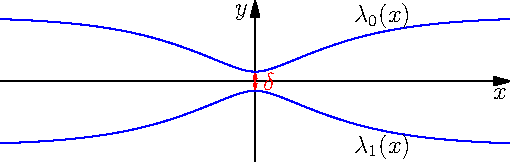
\includegraphics[scale=0.8]{./potential.pdf}
  \end{center}
  \begin{itemize}
  \item $\Ket{\Psi}$ is a vector
  \end{itemize}
\end{frame}


\begin{frame}{Time-dependent Schrödinger equation}{Initial values}
  \begin{center}
    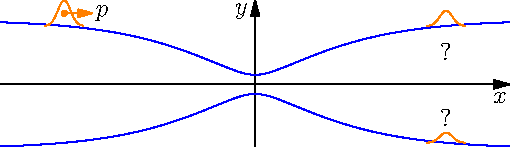
\includegraphics[scale=0.8]{./iv.pdf}
  \end{center}
  \begin{itemize}
  \item Put a wavepacket $\Ket{\Psi}$ somewhere
  \item Add an initial impulse
  \item See what happens at (and after) the avoided crossing
  \end{itemize}
\end{frame}


\section{Operator Splitting}


\begin{frame}{Analytical solution and operator splitting method}
  \begin{itemize}
  \item Analytical solution available but useless
  \end{itemize}
  \begin{equation*} \label{eq:basics_analytic_time_propagation}
    \begin{split}
      \Ket{\psi\ofs{t}} & = e^{- \frac{i}{\varepsilon^2} H t } \Ket{\psi\ofs{0}} = \exp\ofs{\frac{-i}{\varepsilon^2}T t + \frac{-i}{\varepsilon^2}V t} \Ket{\psi\ofs{0}} \\
    \end{split}
  \end{equation*}
  \begin{itemize}
  \item Solution:
    \begin{itemize}
    \item Time evolution by a symmetric Lie-Trotter splitting of $H$
    \item Unitary propagator
    \item State-of-the-art method, is called the \emph{exact solution}
    \end{itemize}
  \end{itemize}
\end{frame}


\begin{frame}{Operator splitting method}{Time stepping and numerical issues}
  A single time step $\tau$:
  \begin{equation*}
    \Ket{\psi\ofs{t+\tau}} = e^{-\frac{i}{2\varepsilon^2} \tau V\ofs{x}} \ift{  e^{-\frac{i}{\varepsilon^2} \tau T\ofs{\omega}} \ft{ e^{-\frac{i}{2\varepsilon^2} \tau V\ofs{x}} \Ket{\psi\ofs{x,t}}}}
  \end{equation*}
  \begin{itemize}
  \item Compute matrix exponential
    \begin{itemize}
    \item of $V$ in position space
    \item of $T$ in momentum space
    \end{itemize}
  \end{itemize}
  \begin{itemize}
  \item Solution can be highly oscillatory!
  \item Need a very fine $\bigO{\varepsilon^2}$ grid on the whole domain
  \item Boundary effects due to Fourier Transformation
  \end{itemize}
\end{frame}


\section{Semiclassical wavepackets}


\begin{frame}{Semiclassical wavepackets}{Definition of the basis functions}
  \begin{itemize}
  \item Basis functions: product of a Gaussian times a polynomial
  \end{itemize}
  \begin{equation*} \label{eq:hagedorn_groundstate_1d}
    \phi_0 \ofs{x} \assign
    \left(\pi\varepsilon^2\right)^{-\frac{1}{4}} Q^{-\frac{1}{2}}
    \exp \left(
      \frac{i}{2\varepsilon^2} PQ^{-1}\left(x-q\right)^2
      + \frac{i}{\varepsilon^2} p\left(x-q\right)
    \right)
  \end{equation*}
  \begin{itemize}
  \item Construct $\phi_k$ by applying the \emph{raising operator} $\mathcal{R}$
  \end{itemize}
  \begin{equation*} \label{eq:definition_ladder_ops}
    \mathcal{R} = \frac{i}{\sqrt{2\varepsilon^2}} \left( \conj{P} \left(x-q\right) + i \varepsilon^2 \conj{Q} \left( \frac{\partial}{\partial x}-p\right) \right)
  \end{equation*}
  \begin{itemize}
  \item We get then
  \end{itemize}
  \begin{equation*}
    \phi_k \assign \frac{1}{\sqrt{k!}} \mathcal{R}^k \phi_0
  \end{equation*}
\end{frame}


\begin{frame}{Semiclassical wavepackets}{Definition of a wavepacket}
  \begin{itemize}
  \item General state on one energy level as linear combination
  \end{itemize}
  \begin{equation*} \label{eq:hawp_def_single}
    \Phi\of{x} \assign e^{\frac{iS}{\varepsilon^2}} \sum_{k=0}^{K-1} c_k \phi_k \of{x}
  \end{equation*}
  \begin{itemize}
  \item We need a vector of multiple $\Phi$
  \item Global parameter set $\Pi \assign \{P, Q, S, p, q\}$
  \item Individual coefficients $c \assign \left(c_0, \ldots, c_{K-1}\right)\T$
  \end{itemize}
  \begin{align*} \label{eq:hawp_def_state_vector}
    \Ket{\Psi} & \assign \Ket{ \begin{pmatrix}
        \Phi_0\of{x} \\
        \vdots \\
        \Phi_{N-1}\of{x} \\
      \end{pmatrix}}
  \end{align*}
\end{frame}


\section{Propagation of semiclassical wavepackets}


\begin{frame}{Theorems about exact propagation}
  Plug $\Ket{\Psi}$ into the TDSE and propagate \\~ \\
  \begin{itemize}
  \item Exact propagation only changes the values of $\Pi$
  \item We have exact propagation iff
    \begin{itemize}
    \item $H = T$
    \item $H = U$ where $U$ is quadratic
    \end{itemize}
  \item Otherwise: propagation changes the values of $c$
    \begin{itemize}
    \item $H = W$ where $W = V - U$ is the non-quadratic remainder
    \end{itemize}
  \item Split the Schrödinger equation and propagate by $T$, $U$ and $W$ separately
  \end{itemize}
\end{frame}


\begin{frame}{The algorithm}
  \begin{algorithmic}
    \REQUIRE A semiclassical wavepacket $\Ket{\Psi\ofs{t}}$
    \REQUIRE The set $\Pi$ of Hagedorn parameters of $\Psi$
    \STATE // Propagate with the kinetic operator
    \STATE $q^{\left(j+\frac{1}{2}\right)} \assign q^{\left(j\right)} + \frac{\tau}{2} p^{\left(j\right)}$
    \STATE $Q^{\left(j+\frac{1}{2}\right)} \assign Q^{\left(j\right)} + \frac{\tau}{2} P^{\left(j\right)}$
    \STATE $S^{\left(j+\frac{1}{2},-\right)} \assign S^{\left(j\right)} + \frac{\tau}{4} p^{\left(j\right)}\T p^{\left(j\right)}$
    \STATE // Propagate with the local quadratic potential
    \STATE $p^{\left(j+1\right)} \assign p^{\left(j\right)} - \tau \, \nabla \lambda_\chi\ofs{q^{\left(j+1/2\right)}}$
    \STATE $P^{\left(j+1\right)} \assign P^{\left(j\right)} - \tau \, \nabla^2 \lambda_\chi\ofs{q^{\left(j+1/2\right)}} Q^{\left(j+1/2\right)}$
    \STATE $S^{\left(j+1/2,+\right)} \assign S^{\left(j+1/2,-\right)} - \tau \, \lambda_\chi\ofs{q^{\left(j+1/2\right)}}$
    \STATE // Propagate with the non-quadratic remainder
  \end{algorithmic}
\end{frame}


\begin{frame}{The algorithm, continued}
  \begin{algorithmic}
    \STATE // Stack the coefficient vectors $c^n$ of all components
    \STATE $C^{\left(j\right)} \assign \left(c^0, \hdots, c^{N-1}\right)\T$
    \STATE // Assemble the block matrix $\mathbf{F}$
    \STATE $\mathbf{F}^{\left(j+1/2\right)} \assign \left(F_{r,c}\right)_{r,c} \quad \forall r,c \in 0,\ldots,N-1$
    \STATE // Propagate the coefficients
    \STATE $C^{\left(j+1\right)} \assign \exp\ofs{-\tau \frac{i}{\varepsilon^2} \mathbf{F}^{\left(j+1/2\right)}} C^{\left(j\right)}$
    \STATE // Split the coefficients
    \STATE $\left(c^0, \ldots, c^{N-1}\right) \assign C^{\left(j+1\right)}$
    \STATE // Propagate with the kinetic operator again
    \STATE $q^{\left(j+1\right)} \assign q^{\left(j+1/2\right)} + \frac{\tau}{2} p^{\left(j+1\right)}$
    \STATE $Q^{\left(j+1\right)} \assign Q^{\left(j+1/2\right)} + \frac{\tau}{2} P^{\left(j+1\right)}$
    \STATE $S^{\left(j+1\right)} \assign S^{\left(j+1/2,+\right)} + \frac{\tau}{4} p^{\left(j+1\right)}\T p^{\left(j+1\right)}$
    \RETURN $\Ket{\Psi\ofs{t+\tau}}$
  \end{algorithmic}
\end{frame}


\subsection{Advantages of wavepackets}


\begin{frame}{Some final remarks}
  \begin{itemize}
  \item Wavepackts work very well for simple potentials
  \item Some open issues for more complex potentials
    \begin{itemize}
    \item Several parameters to choose, for example the basis size
    \end{itemize}
  \item Gridless method
    \begin{itemize}
    \item but we need very high order quadrature
    \item and the matrix exponential of a full matrix
    \end{itemize}
  \item Unbounded domains possible
  \end{itemize}
\end{frame}


\section{Examples}


\begin{frame}{Two energy levels with a single avoided crossing}
  \begin{equation*}
    V\ofs{x} =   \frac{1}{2}
    \begin{pmatrix}
      \tanh(x) & \delta \\
      \delta   & -\tanh(x)
    \end{pmatrix}
  \end{equation*}
  \begin{align*}
    \varepsilon & = 0.2 \\
    \delta & = 0.5 \cdot \varepsilon \\
    \Ket{\Psi} & = \Ket{ \begin{pmatrix}
        \phi_2\of{x} \\
        0
      \end{pmatrix}} \\
    \Pi & = \{P, Q, S, p, q\} = \{1.0i, 1.0-6.0i, 0.0, 1.0, -6.0\}
  \end{align*}
\end{frame}


\begin{frame}{Two avoided crossings in series}
  \begin{equation*}
    V\ofs{x} =
    \frac{1}{2}
    \begin{pmatrix}
      \Theta & \delta \\
      \delta & -\Theta
    \end{pmatrix}
  \end{equation*}
  where
  \begin{equation*}
    \Theta \assign \tanh(x-\rho) \tanh(x+\rho)
  \end{equation*}
  and $\rho = 3.0$
\end{frame}


\begin{frame}{Three energy levels with multiple avoided crossings}
  \begin{equation*}
    V\ofs{x} = \begin{pmatrix}
      \Theta + \Xi & \delta_1 & \delta_2 \\
      \delta_1     & -\Theta  & 0 \\
      \delta_2     & 0        & 1 - \Xi
    \end{pmatrix}
  \end{equation*}
  where
  \begin{equation*}
    \Theta \assign \tanh(x + \rho) \quad \text{and} \quad
    \Xi \assign \tanh(x-\rho)
  \end{equation*}
  and $\rho = 3.0$
\end{frame}


\section{Current and future work}


\begin{frame}{Current and future work}{An active topic of research}
  \begin{itemize}
  \item Improve for more complicated potentials, more energy levels
    \begin{itemize}
    \item Spawning of new packets during simulation
    \item Multiple parameter sets $\Pi$
    \end{itemize}
  \item Find evidence (or proof) for conjectures about convergence
  \item Go to higher dimensional space
    \begin{itemize}
    \item Sparse packets for reducing the number of coefficients $c$
    \end{itemize}
  \item \ldots
  \item Much more interesting work!
  \end{itemize}
\end{frame}


\section{End}


\begin{frame}{Thanks for your attention}
  More information on the topic
  \begin{itemize}
  \item The full thesis:\\
    {\burl{http://www.sam.math.ethz.ch/~raoulb/research/bachelor_thesis/tex/main.pdf}}
  \item More simulation results:\\
    {\burl{http://www.sam.math.ethz.ch/~raoulb/research/bachelor_thesis}}
  \item The python source code (outdated):\\
    {\burl{https://github.com/raoulbq/WaveBlocks}}
  \end{itemize}
  \begin{center}
    
\includegraphics[scale=1.0]{./python-powered-w.pdf}
  \end{center}
\end{frame}

\end{document}
